\documentclass[11pt,]{article}

\usepackage{pandoc/iclc}

\usepackage{amssymb,amsmath}
\usepackage{ifxetex,ifluatex}
\usepackage{fixltx2e} % provides \textsubscript
\ifnum 0\ifxetex 1\fi\ifluatex 1\fi=0 % if pdftex
    \usepackage{inconsolata}
  \usepackage{inconsolata}
    \usepackage[T1]{fontenc}
  \usepackage[utf8]{inputenc}
\else % if luatex or xelatex
  \ifxetex
    \usepackage{mathspec}
    \usepackage{xltxtra,xunicode}
  \else
    \usepackage{fontspec}
  \fi
  \defaultfontfeatures{Mapping=tex-text,Scale=MatchLowercase}
  \newcommand{\euro}{€}
    \setmainfont{Linux Libertine}
    \setmonofont[Mapping=tex-ansi]{Inconsolata}
\fi
% use upquote if available, for straight quotes in verbatim environments
\IfFileExists{upquote.sty}{\usepackage{upquote}}{}
% use microtype if available
\IfFileExists{microtype.sty}{%
\usepackage{microtype}
\UseMicrotypeSet[protrusion]{basicmath} % disable protrusion for tt fonts
}{}
\usepackage[margin=2cm]{geometry}
\usepackage{color}
\usepackage{fancyvrb}
\newcommand{\VerbBar}{|}
\newcommand{\VERB}{\Verb[commandchars=\\\{\}]}
\DefineVerbatimEnvironment{Highlighting}{Verbatim}{commandchars=\\\{\}}
% Add ',fontsize=\small' for more characters per line
\newenvironment{Shaded}{}{}
\newcommand{\AlertTok}[1]{\textcolor[rgb]{1.00,0.00,0.00}{\textbf{#1}}}
\newcommand{\AnnotationTok}[1]{\textcolor[rgb]{0.38,0.63,0.69}{\textbf{\textit{#1}}}}
\newcommand{\AttributeTok}[1]{\textcolor[rgb]{0.49,0.56,0.16}{#1}}
\newcommand{\BaseNTok}[1]{\textcolor[rgb]{0.25,0.63,0.44}{#1}}
\newcommand{\BuiltInTok}[1]{\textcolor[rgb]{0.00,0.50,0.00}{#1}}
\newcommand{\CharTok}[1]{\textcolor[rgb]{0.25,0.44,0.63}{#1}}
\newcommand{\CommentTok}[1]{\textcolor[rgb]{0.38,0.63,0.69}{\textit{#1}}}
\newcommand{\CommentVarTok}[1]{\textcolor[rgb]{0.38,0.63,0.69}{\textbf{\textit{#1}}}}
\newcommand{\ConstantTok}[1]{\textcolor[rgb]{0.53,0.00,0.00}{#1}}
\newcommand{\ControlFlowTok}[1]{\textcolor[rgb]{0.00,0.44,0.13}{\textbf{#1}}}
\newcommand{\DataTypeTok}[1]{\textcolor[rgb]{0.56,0.13,0.00}{#1}}
\newcommand{\DecValTok}[1]{\textcolor[rgb]{0.25,0.63,0.44}{#1}}
\newcommand{\DocumentationTok}[1]{\textcolor[rgb]{0.73,0.13,0.13}{\textit{#1}}}
\newcommand{\ErrorTok}[1]{\textcolor[rgb]{1.00,0.00,0.00}{\textbf{#1}}}
\newcommand{\ExtensionTok}[1]{#1}
\newcommand{\FloatTok}[1]{\textcolor[rgb]{0.25,0.63,0.44}{#1}}
\newcommand{\FunctionTok}[1]{\textcolor[rgb]{0.02,0.16,0.49}{#1}}
\newcommand{\ImportTok}[1]{\textcolor[rgb]{0.00,0.50,0.00}{\textbf{#1}}}
\newcommand{\InformationTok}[1]{\textcolor[rgb]{0.38,0.63,0.69}{\textbf{\textit{#1}}}}
\newcommand{\KeywordTok}[1]{\textcolor[rgb]{0.00,0.44,0.13}{\textbf{#1}}}
\newcommand{\NormalTok}[1]{#1}
\newcommand{\OperatorTok}[1]{\textcolor[rgb]{0.40,0.40,0.40}{#1}}
\newcommand{\OtherTok}[1]{\textcolor[rgb]{0.00,0.44,0.13}{#1}}
\newcommand{\PreprocessorTok}[1]{\textcolor[rgb]{0.74,0.48,0.00}{#1}}
\newcommand{\RegionMarkerTok}[1]{#1}
\newcommand{\SpecialCharTok}[1]{\textcolor[rgb]{0.25,0.44,0.63}{#1}}
\newcommand{\SpecialStringTok}[1]{\textcolor[rgb]{0.73,0.40,0.53}{#1}}
\newcommand{\StringTok}[1]{\textcolor[rgb]{0.25,0.44,0.63}{#1}}
\newcommand{\VariableTok}[1]{\textcolor[rgb]{0.10,0.09,0.49}{#1}}
\newcommand{\VerbatimStringTok}[1]{\textcolor[rgb]{0.25,0.44,0.63}{#1}}
\newcommand{\WarningTok}[1]{\textcolor[rgb]{0.38,0.63,0.69}{\textbf{\textit{#1}}}}
% definitions for citeproc citations
\NewDocumentCommand\citeproctext{}{}
\NewDocumentCommand\citeproc{mm}{%
  \begingroup\def\citeproctext{#2}\cite{#1}\endgroup}
\makeatletter
 % allow citations to break across lines
 \let\@cite@ofmt\@firstofone
 % avoid brackets around text for \cite:
 \def\@biblabel#1{}
 \def\@cite#1#2{{#1\if@tempswa , #2\fi}}
\makeatother
\newlength{\cslhangindent}
\setlength{\cslhangindent}{1.5em}
\newlength{\csllabelwidth}
\setlength{\csllabelwidth}{3em}
\newenvironment{CSLReferences}[2] % #1 hanging-indent, #2 entry-spacing
 {\begin{list}{}{%
  \setlength{\itemindent}{0pt}
  \setlength{\leftmargin}{0pt}
  \setlength{\parsep}{0pt}
  % turn on hanging indent if param 1 is 1
  \ifodd #1
   \setlength{\leftmargin}{\cslhangindent}
   \setlength{\itemindent}{-1\cslhangindent}
  \fi
  % set entry spacing
  \setlength{\itemsep}{#2\baselineskip}}}
 {\end{list}}
\usepackage{calc}
\newcommand{\CSLBlock}[1]{\hfill\break\parbox[t]{\linewidth}{\strut\ignorespaces#1\strut}}
\newcommand{\CSLLeftMargin}[1]{\parbox[t]{\csllabelwidth}{\strut#1\strut}}
\newcommand{\CSLRightInline}[1]{\parbox[t]{\linewidth - \csllabelwidth}{\strut#1\strut}}
\newcommand{\CSLIndent}[1]{\hspace{\cslhangindent}#1}
\usepackage{graphicx}
\makeatletter
% pandoc version < 3.2
\def\maxwidth{\ifdim\Gin@nat@width>\linewidth\linewidth\else\Gin@nat@width\fi}
\def\maxheight{\ifdim\Gin@nat@height>\textheight\textheight\else\Gin@nat@height\fi}
% Scale images if necessary, so that they will not overflow the page
% margins by default, and it is still possible to overwrite the defaults
% using explicit options in \includegraphics[width, height, ...]{}
\setkeys{Gin}{width=\maxwidth,height=\maxheight,keepaspectratio}
% pandoc version > 3.2
\newsavebox\pandoc@box
\newcommand*\pandocbounded[1]{% scales image to fit in text height/width
  \sbox\pandoc@box{#1}%
  \Gscale@div\@tempa{\textheight}{\dimexpr\ht\pandoc@box+\dp\pandoc@box\relax}%
  \Gscale@div\@tempb{\linewidth}{\wd\pandoc@box}%
  \ifdim\@tempb\p@<\@tempa\p@\let\@tempa\@tempb\fi% select the smaller of both
  \ifdim\@tempa\p@<\p@\scalebox{\@tempa}{\usebox\pandoc@box}%
  \else\usebox{\pandoc@box}%
  \fi%
}
\makeatother
\ifxetex
  \usepackage[setpagesize=false, % page size defined by xetex
              unicode=false, % unicode breaks when used with xetex
              xetex]{hyperref}
\else
  \usepackage[unicode=true]{hyperref}
\fi
\hypersetup{breaklinks=true,
            bookmarks=true,
            pdfauthor={},
            pdftitle={KabelSalat: Live Coding Audio-Visual Graphs on the Web and Beyond},
            colorlinks=true,
            citecolor=blue,
            urlcolor=blue,
            linkcolor=magenta,
            pdfborder={0 0 0}}
\urlstyle{same}  % don't use monospace font for urls
\setlength{\parindent}{0pt}
\setlength{\parskip}{6pt plus 2pt minus 1pt}
\setlength{\emergencystretch}{3em}  % prevent overfull lines
\providecommand{\tightlist}{%/
  \setlength{\itemsep}{0pt}\setlength{\parskip}{0pt}}
\setcounter{secnumdepth}{5}

\title{KabelSalat: Live Coding Audio-Visual Graphs on the Web and
Beyond}
\author{
  Felix Roos \\
  Unaffiliated\\
  \href{mailto:flix91@gmail.com}{flix91@gmail.com}
   \and 
  Raphaël Maurice Forment \\
  Université Jean Monnet\\
  \href{mailto:raphael.forment@gmail.com}{raphael.forment@gmail.com}
  }
\date{}
\usepackage{svg}

\begin{document}
\maketitle
\begin{abstract}
This paper introduces KabelSalat, a graph-based live coding environment
that targets multiple platforms and languages. It works by translating a
Domain Specific Language (DSL) based on JavaScript into a signal flow
graph. This graph can be compiled into a sequence of instructions
optimized for real time signal processing. The DSL has been implemented
both in JavaScript and Lua. The compiler can either output JavaScript
code to run in the browser or optimized C code to run natively. The
possibility of adding other target languages is an integral part of
KabelSalat's design. The browser version includes a REPL and features a
range of audio DSP nodes reminiscent of modular synthesizers. Notable
features include single sample feedback and multi-channel expansion
inspired by the SuperCollider audio engine. The core module of
KabelSalat has also been used to implement a stripped down version of
the Hydra video synthesizer, thus demonstrating that the same underlying
principles can be adapted both for audio and video generation. In the
future, KabelSalat might become an alternative audio engine for Strudel,
offering more sound design capabilities, compared to the current
superdough engine, which uses the browser's built-in Web Audio Nodes.
\end{abstract}

\pandocbounded{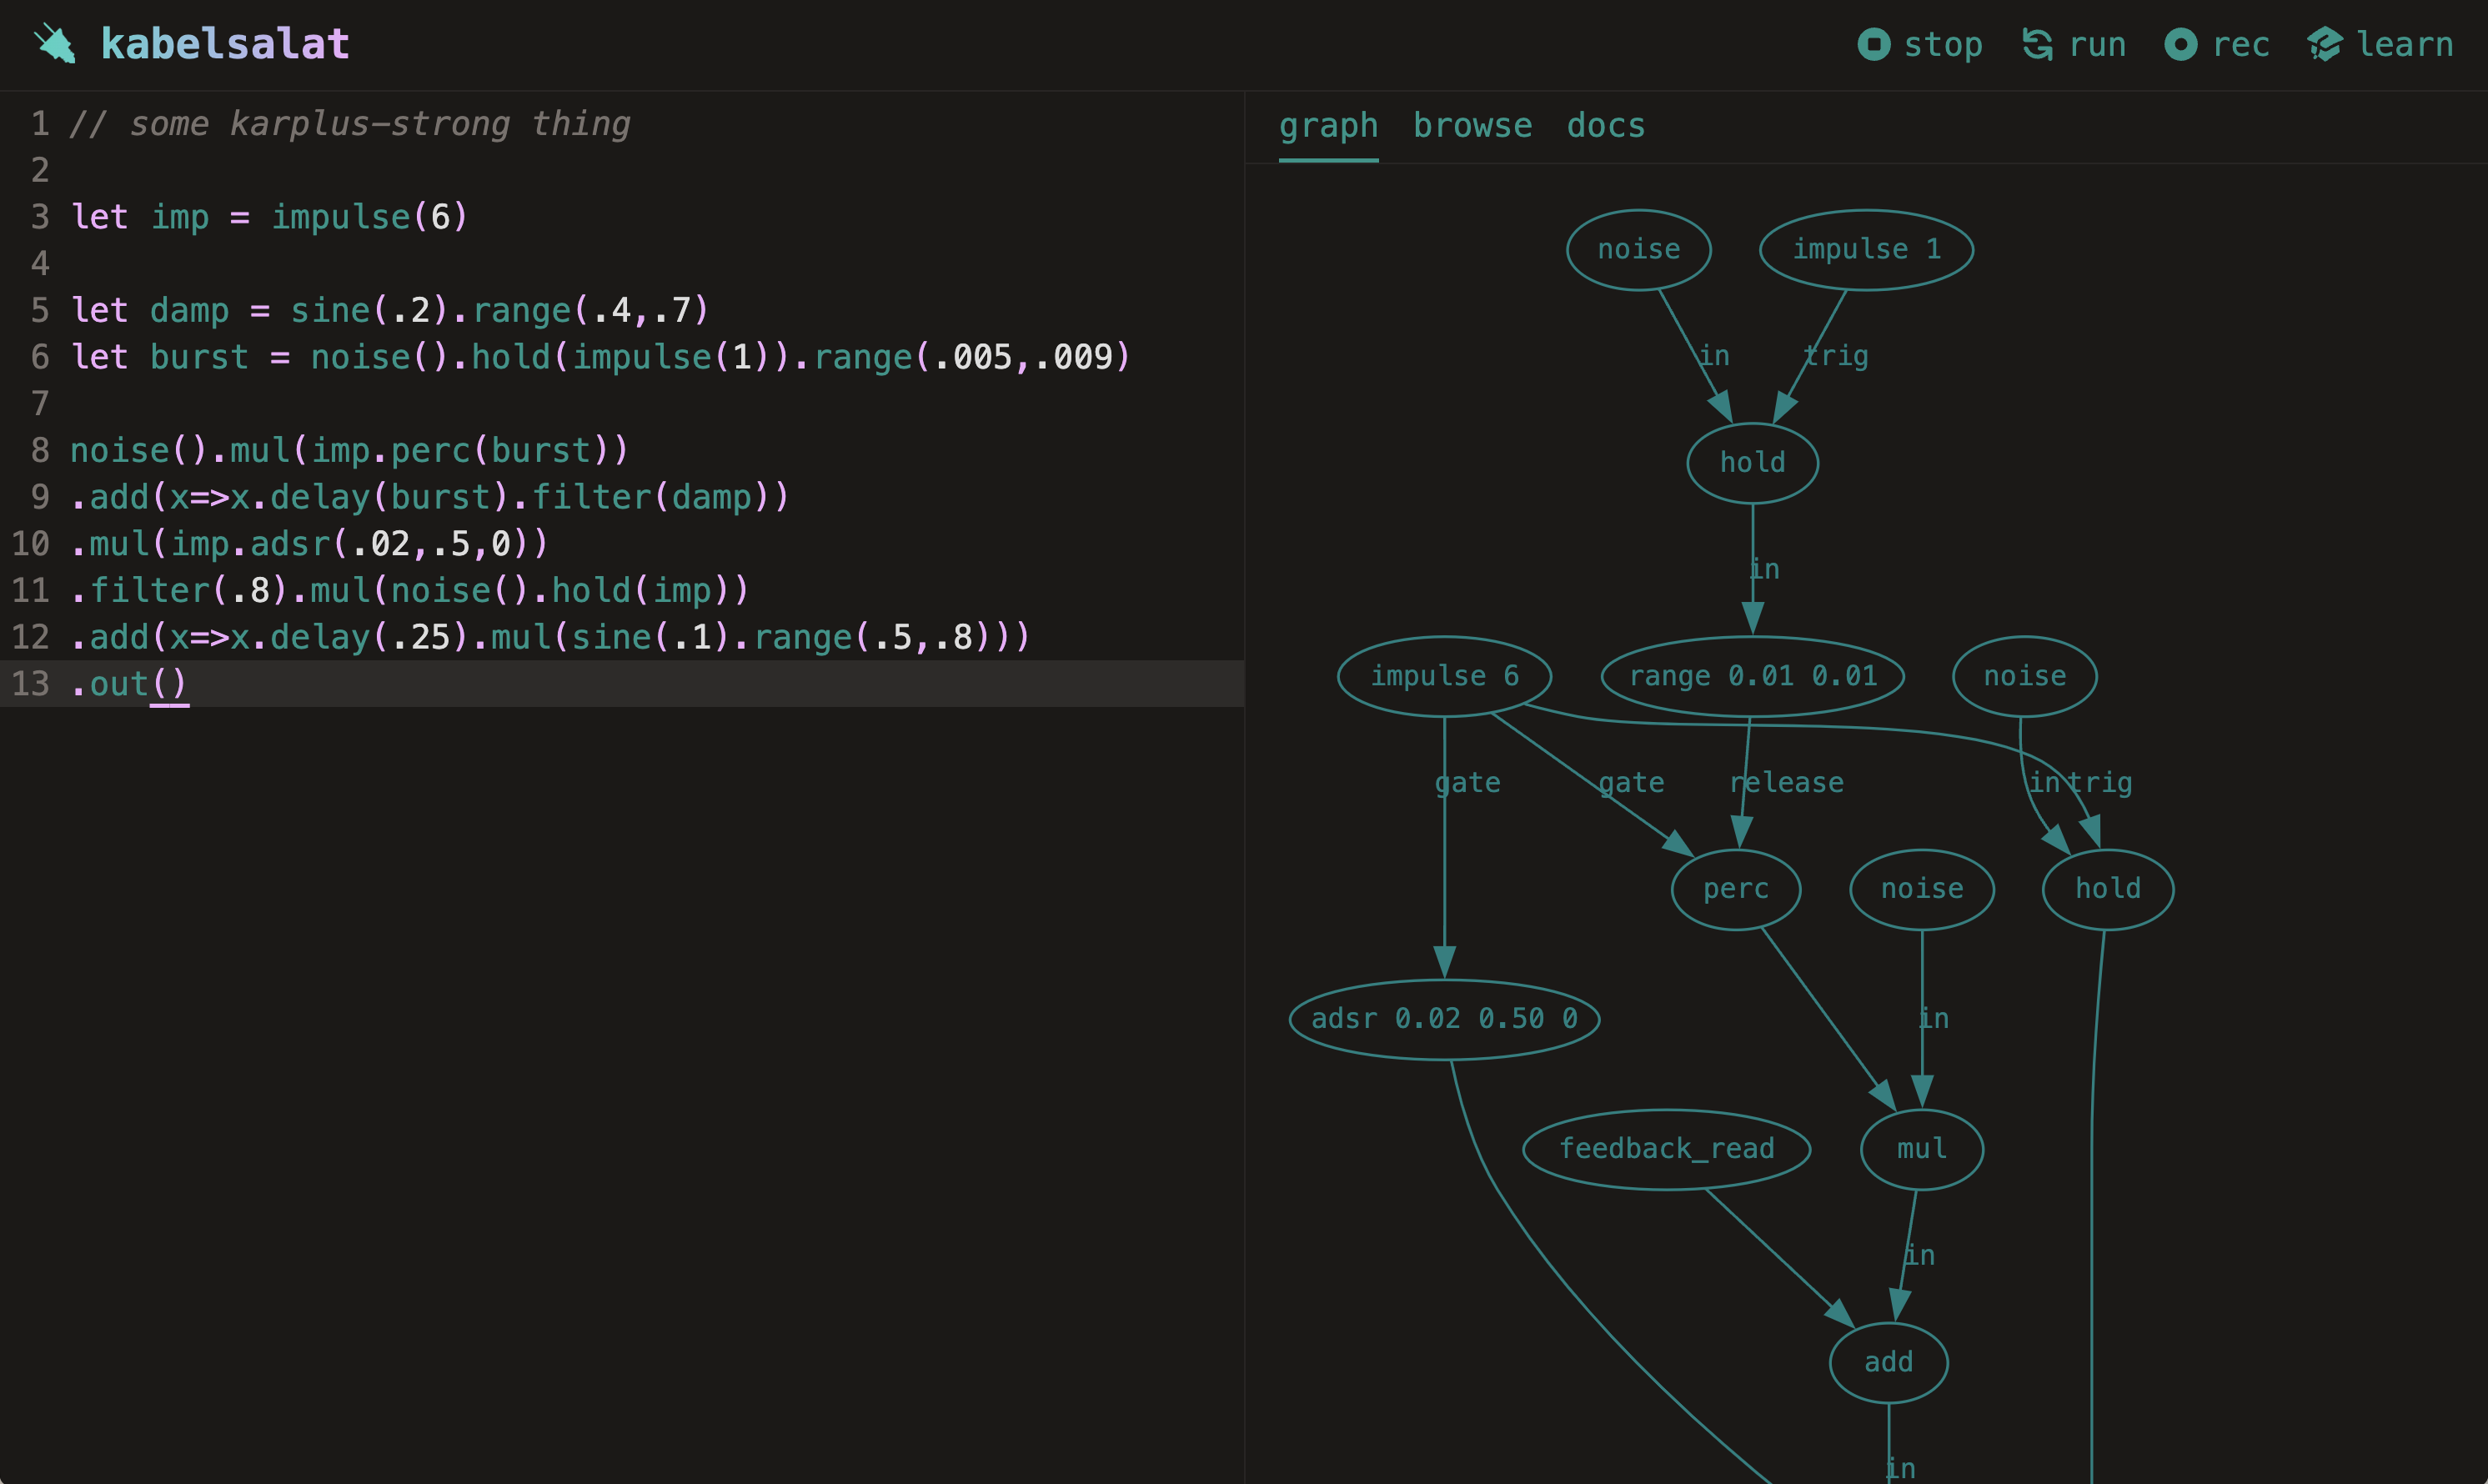
\includegraphics[keepaspectratio]{images/kabelsalat_full.png}}
Figure 1: KabelSalat web interface (\url{https://kabel.salat.dev},
accessed on September 27, 2024) running a Karplus Strong patch. On the
left pane pane: source code editor. On the right pane: audio graph
visualizer. \pagebreak

\section{Introduction}\label{introduction}

Graphs are often used to represent the signal flow of live coding
systems, as demonstrated by Glicol (Lan and Jensenius 2021), Genish.js
(Roberts 2017), Hydra (Jack 2018) or Punctual (Ogborn 2018). Using
graph-based data structures, logic and/or user interfaces is a common
paradigm for all creative software that preferably direct information
and data according to this metaphor, encompassing both audio and
image/video applications. The same reason explains the popularity of
this paradigm in live patching environments such as NoiseCraft
(Chevalier-Boisvert 2021), cables.gl (Kombuechen 2020) or VCVRack.
Graphs are sometimes perceived as more natural to the end user. They
allow a direct and intuitive representation of the signal flow,
sometimes emulating the patching of pedalboards or modular synthesizers.
Many important audio programming languages from the past decades, such
as Pure Data (Puckette 1996) and SuperCollider (McCartney 2002) are also
computing audio based on the concept of signal flow graphs. In this
specific case, the reason for using graphs is quite different. Graphs
often allow for an optimized execution of the signal processing chain,
as they can be analyzed and optimized before execution.

Digital signal processing in web browsers has historically adopted a
graph based approach, as demonstrated by the Web Audio API\footnote{The
  \emph{Mozilla Developer Network} website provides a thorough
  introduction to the Web Audio API:
  \url{https://developer.mozilla.org/en-US/docs/Web/API/Web_Audio_API/Using_Web_Audio_API}
  (accessed on September 27, 2024). This API can be considered as the
  basic building blocks for more complex applications and libraries such
  as ToneJS (Mann 2015).}. This \emph{dataflow paradigm} continues to
gain in popularity in the context of Web Audio. The Web Audio API is
based on a classic block-based processing model (Roads 1996) and relies
on a set of predefined audio nodes comparable to UGens in computer music
programming languages. These nodes are designed for lightweight
multimedia applications rather than specialized audio and signal
processing (\emph{e.g.} basic audio filters, equalization, panning)
where time and CPU usage are a critical resource. For the creative
musicians, such nodes can be limiting, as they do not allow for the
creation of complex audio graphs or the implementation of optimized and
lightweight specialized audio algorithms. The introduction of
AudioWorklets has recently opened up the possibility of single-sample
processing in the browser (Choi 2018). They also offer a way for
developers to build bespoke audio nodes. AudioWorklets are offering
significant advantages over block-based processing. Single-sample
processing removes the block size constraint of classic Web Audio nodes,
which is often felt as both a technical and creative limitation.
Computing audio in blocks can prevent or hinder the implementation of
various classic algorithms: filter design, physical modeling, etc.
Consequently, this can have an incidence on the sonic palette available
to the musician. Despite their recent introduction, AudioWorklets have
already proven their value in the implementation of audio feedback
loops, granular synthesis algorithms (Roberts 2017, 2018) or physical
modeling (ADD EXAMPLE). AudioWorklets are offering yet another
advantage: they are self-contained signal processors that do not depend
on web platform specifics. They be developed in JavaScript and/or
compiled to WebAssembly from any other language supporting this
compilation target.

We began exploring the new avenues introduced by AudioWorklets because
of technical and creative constraints felt during the development of
Strudel (Roos and McLean 2023). Strudel audio engine,
\emph{SuperDough}\footnote{Link to \emph{SuperDough} on the \emph{npm}
  package manager: \url{https://www.npmjs.com/package/superdough}
  (accessed on September 27, 2024).}, is built using the aforementioned
Web Audio API. It is built in imitation to \emph{SuperDirt}, the classic
Tidal Cycles audio engine, that relies on the extensive capabilities of
the SuperCollider audio server\footnote{Link to the \emph{SuperDit}
  repository on GitHub:
  \url{https://github.com/musikinformatik/SuperDirt} (\emph{idem}).}. In
order to provide users with a similar level of flexibility and
expressiveness in audio design, we needed to find a way to implement
high-performance custom audio nodes in the browser. Our long-term goal
is to be able to replace Strudel's current audio engine, called
\emph{SuperDough}, by a custom and flexible solution based on
AudioWorklets. For the time being, Strudel still uses the more limited
set of features provided by the Web Audio API nodes.

\section{Introducing the KabelSalat
DSL}\label{introducing-the-kabelsalat-dsl}

KabelSalat implements a Domain Specific Language (DSL) to represent and
compile graphs suitable for single-sample processing. It can be used
both a prototyping bench for audio algorithms or as a DSP-oriented live
coding language.~The KabelSalat compiler and runtime is designed, above
all things, to be embedded in other applications. However, it can also
be used as a standalone application through an Integrated Development
Environment (see Figure 1). The compilation strategy -- as well as many
fundamental audio nodes -- are based on the browser-based NoiseCraft
synthesizer (Chevalier-Boisvert 2021). KabelSalat's development started
via an attempt to rewrite NoiseCraft's compiler to a version that
encapsulates its core logic from the output language, allowing each node
to control its own code generation (UNCLEAR, ADD FOOTNOTE). With this
crucial addition, the core language is not specifically tied to a
specific audio graph format or to a single target language. To test the
viability of this design, we have developed a way for KabelSalat patches
to be compiled to C code and played as standalone binaries. As another
proof-of-concept, KabelSalat was used to compile Hydra patches to GLSL
code (Jack 2018), showing an application of the same concepts in another
neighbouring domain.

\newpage

\subsection{First example: a substractive synthesizer
patch}\label{first-example-a-substractive-synthesizer-patch}

KabelSalat is based on a terse and practical syntax that relies heavily
on method chaining. This can be seen as a way to emulate the patch point
connexions between the different modules of a synthesizer. Functions and
methods can be considered as signal generators or processors (nodes),
which can be connected and/or combined to other modules through chaining
or reference. Arguments of these nodes can either be constant values or
other nodes\footnote{}. The same basic principles can be used for
creating patches of arbitrary depth and complexity. Figure 2 and 3
provide an example of how a classic subtractive synthesizer patch can be
written in KabelSalat, and how a visual trace of the audio graph can be
generated in real time.

\vspace{0.5em}
\setcounter{figure}{1}    
\begin{figure}[h!]
    \centering
    \begin{minipage}{0.40\textwidth}
        \begin{Shaded}
        \begin{Highlighting}[]
        \CommentTok{// sawtooth wave at 55Hz:}
        \FunctionTok{saw}\NormalTok{(}\DecValTok{55}\NormalTok{)}
          \CommentTok{// modulated low{-}pass{-}filter}
          \OperatorTok{.}\FunctionTok{lpf}\NormalTok{(}\FunctionTok{sine}\NormalTok{(}\DecValTok{1}\NormalTok{)}\OperatorTok{.}\FunctionTok{range}\NormalTok{(}\FloatTok{0.4}\OperatorTok{,} \FloatTok{0.8}\NormalTok{))}
          \CommentTok{// modulated amplitude:}
          \OperatorTok{.}\FunctionTok{mul}\NormalTok{(}\FunctionTok{sine}\NormalTok{(}\DecValTok{4}\NormalTok{)}\OperatorTok{.}\FunctionTok{range}\NormalTok{(}\FloatTok{0.25}\OperatorTok{,} \DecValTok{1}\NormalTok{))}
          \CommentTok{// send to audio output:}
          \OperatorTok{.}\FunctionTok{out}\NormalTok{()}\OperatorTok{;}
        \end{Highlighting}
        \end{Shaded}
        \caption{A low-pass filtered sawtooth oscillator with a final stage of amplitude modulation.}
    \end{minipage}\hspace{0.1\textwidth}
    \begin{minipage}{0.40\textwidth}
        \centering
        \pandocbounded{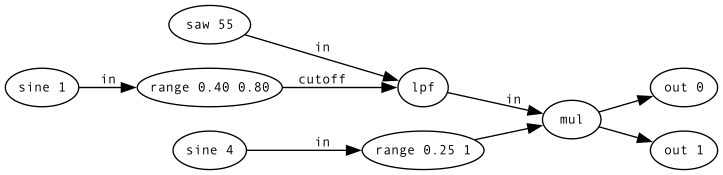
\includegraphics[keepaspectratio]{images/figure1.png}}
        \vspace{4.2em}
        \caption{Visual representation of the same audio graph, generated in real-time using GraphViz.}
    \end{minipage}
\end{figure}

\subsection{Method Chaining}\label{method-chaining}

The previous example implicitely demonstrates how KabelSalat
\emph{flattens} the syntax in order to make the code more readable to
the end-user. Figure 4 reproduces the same patch, using only function
calls. Even though the code appears syntactically simpler, it becomes
more difficult to parse and manipulate for musicians in the context of a
live coding session. Method chaining cna be seen as a way to alleviate
this issue. Similar to Hydra (Jack 2018) and Strudel (Roos and McLean
2023)\footnote{Strudel used the same technique applied to a different
  domain: the functional composition of musical patterns. Hydra uses it,
  similarly to KabelSalat, as a way to connect and combine video
  processing nodes.}, it has been designed to work in a similar fashion
to infix notation, without the need to overload operators. When a method
is called on a node, that node is used as the first input of the method.
Method chaining provides a visual linearity that is often advantegeous
for parsing and editing code representing signal flows.

\begin{Shaded}
\begin{Highlighting}[]
\CommentTok{// send to output:}
\FunctionTok{out}\NormalTok{(}
  \CommentTok{// modulate amplitude}
  \FunctionTok{mul}\NormalTok{(}
    \CommentTok{// modulated low{-}pass{-}filter}
    \FunctionTok{lpf}\NormalTok{(}
      \CommentTok{// sawtooth wave at 55Hz:}
      \FunctionTok{saw}\NormalTok{(}\DecValTok{55}\NormalTok{)}\OperatorTok{,}
      \FunctionTok{range}\NormalTok{(}\FunctionTok{sine}\NormalTok{(}\DecValTok{1}\NormalTok{)}\OperatorTok{,} \FloatTok{0.4}\OperatorTok{,} \FloatTok{0.8}\NormalTok{)}
\NormalTok{    )}\OperatorTok{,}
    \FunctionTok{range}\NormalTok{(}\FunctionTok{sine}\NormalTok{(}\DecValTok{2}\NormalTok{)}\OperatorTok{,} \FloatTok{0.25}\OperatorTok{,} \DecValTok{1}\NormalTok{)}
\NormalTok{  )}
\NormalTok{)}\OperatorTok{;}
\end{Highlighting}
\end{Shaded}

Figure 4: The same substractive patch, without using method chaining.
Compared to the method chaining example, the expression is deeply
nested, with a wider distance between logically grouped tokens.
Additionally, editing the expression involves a lot of extra indenting
and cursor movement.

\newpage

\subsection{Multichannel Expansion}\label{multichannel-expansion}

KabelSalat borrows the concept of multichannel expansion from
SuperCollider\footnote{This feature is documented in the official
  SuperCollider documentation:
  \url{https://doc.sccode.org/Guides/Multichannel-Expansion.html}
  (accessed on September 28, 2024).}, allowing the duplication of a node
or a chain of nodes to multiple channels. Large audio graphs involving
parallel processing can thus be generated with relatively few
characters. Multichannel expansion is based on providing function/method
arguments as Arrays (\emph{e.g.} \texttt{{[}1,\ 2,\ 3,\ 4{]}}, see
Figure 4 and 5).

\vspace{0.5em}
\setcounter{figure}{3}    
\begin{figure}[h!]
    \centering
    \begin{minipage}{0.40\textwidth}
        \begin{Shaded}
        \begin{Highlighting}[]
        \CommentTok{// creating two channels of}
        \CommentTok{// filtered sawtooth waves}
        \FunctionTok{saw}\NormalTok{([}\DecValTok{200}\OperatorTok{,} \DecValTok{300}\NormalTok{])}\OperatorTok{.}\FunctionTok{lpf}\NormalTok{(}\FloatTok{0.5}\NormalTok{)}\OperatorTok{.}\FunctionTok{out}\NormalTok{([}\DecValTok{0}\OperatorTok{,} \DecValTok{1}\NormalTok{])}\OperatorTok{;}
        \end{Highlighting}
        \end{Shaded}
        \caption{Multichanel expansion on two channels using Arrays (\texttt{[200, 300]} and \texttt{[0, 1]}).}
    \end{minipage}\hspace{0.1\textwidth}
    \begin{minipage}{0.40\textwidth}
        \centering
        \begin{Shaded}
        \begin{Highlighting}[]
        \CommentTok{// the above is equivalent to:}
        \FunctionTok{saw}\NormalTok{(}\DecValTok{200}\NormalTok{)}\OperatorTok{.}\FunctionTok{lpf}\NormalTok{(}\FloatTok{0.5}\NormalTok{)}\OperatorTok{.}\FunctionTok{out}\NormalTok{(}\DecValTok{0}\NormalTok{)}\OperatorTok{;}
        \FunctionTok{saw}\NormalTok{(}\DecValTok{300}\NormalTok{)}\OperatorTok{.}\FunctionTok{lpf}\NormalTok{(}\FloatTok{0.5}\NormalTok{)}\OperatorTok{.}\FunctionTok{out}\NormalTok{(}\DecValTok{1}\NormalTok{)}\OperatorTok{;}
        \end{Highlighting}
        \end{Shaded}
        \caption{Equivalent code without channel expansion.}
    \end{minipage}
\end{figure}

Multichannel expansion in KabelSalat involves the use of a special
\texttt{poly} node. Each element of the Array used for expansion is
considered as an input. When a node receives a \texttt{poly} node with
\texttt{n} inputs, \texttt{n} copies of the node are created. Each copy
receives one of the values in the Array. The copied nodes are fed into a
new \texttt{poly} node, which is propagated down the graph. The
\texttt{poly} node will eventually end up at the bottom of the graph,
where each channel is assigned to one \texttt{out} node. In cases where
a node receives multiple \texttt{poly} nodes, the \texttt{poly} node
with the most inputs determines the number of copies. The inputs of the
other \texttt{poly} nodes wrap around. Figure 6 shows a graphical
version of how the \texttt{poly} node is propagated in the above
example.

\pandocbounded{\includegraphics[keepaspectratio]{images/mch.png}} Figure
6: compilation stages of the \texttt{poly} node used in Figure 4.

ADD SOMETHING ABOUT THE INTEREST OF MULTICHANNEL EXPANSION FOR USERS /
MUSICIANS

\subsection{Feedback}\label{feedback}

Audio feedback loops plays an important role in digital audio synthesis,
allowing the creation of comb filters, feedback delay networks (FDN),
reverbs, flanger effects, among many other applications (Smith 2010;
Roberts 2017). Feedback is also an important technique in the realm of
video synthesis\footnote{See for instance:
  \url{https://andreijaycreativecoding.com/getting_started-with-video-feedback}
  (accessed September 28, 2024). Feedback loops is also a popular
  feature of the well-known Hydra video synthesizer used by many live
  coders during Algoraves: \url{https://hydra.ojack.xyz/docs/}
  (\emph{idem})}. A feedback loop is created in a graph when a node uses
its own output as an input. KabelSalat supports two techniques to create
such loops: through anonymous functions or through a special
\texttt{source} node.

\newpage

\subsubsection{Feedback loop using anynomous
functions}\label{feedback-loop-using-anynomous-functions}

Passing an anonymous function to any node creates a feedback cycle. In
the example shown in Figure 7, the \texttt{add} node receives an
anonymous function as its input and receives its own output as an
argument. Any alteration or further processing done to the feedback line
can be notated inside the function (\emph{e.g.} amplitude modulation,
introducing an \emph{n} samples delay). Figure 8 illustrates the
representation of a feedback loop in the graph visualizer.

\vspace{0.5em}
\setcounter{figure}{6}    
\begin{figure}[h!]
    \centering
    \begin{minipage}{0.40\textwidth}
        \begin{Shaded}
        \begin{Highlighting}[]
        \FunctionTok{impulse}\NormalTok{(}\DecValTok{1}\NormalTok{)}
          \OperatorTok{.}\FunctionTok{add}\NormalTok{(}
        \NormalTok{    (x) }\KeywordTok{=\textgreater{}}\NormalTok{ x}\OperatorTok{.}\FunctionTok{delay}\NormalTok{(}\FloatTok{0.2}\NormalTok{)}\OperatorTok{.}\FunctionTok{mul}\NormalTok{(}\FloatTok{0.8}\NormalTok{)}
        \NormalTok{  )}
          \OperatorTok{.}\FunctionTok{out}\NormalTok{()}\OperatorTok{;}
        \end{Highlighting}
        \end{Shaded}
        \caption{Introducing a delayed feedback with control over the signal amplitude.}
    \end{minipage}\hspace{0.1\textwidth}
    \begin{minipage}{0.40\textwidth}
        \centering

        \caption{Equivalent code without channel expansion.}
    \end{minipage}
\end{figure}

\begin{Shaded}
\begin{Highlighting}[]
\FunctionTok{impulse}\NormalTok{(}\DecValTok{1}\NormalTok{)}
  \OperatorTok{.}\FunctionTok{add}\NormalTok{(}
\NormalTok{    (x) }\KeywordTok{=\textgreater{}}\NormalTok{ x}\OperatorTok{.}\FunctionTok{delay}\NormalTok{(}\FloatTok{0.2}\NormalTok{)}\OperatorTok{.}\FunctionTok{mul}\NormalTok{(}\FloatTok{0.8}\NormalTok{)}
\NormalTok{  )}
  \OperatorTok{.}\FunctionTok{out}\NormalTok{()}\OperatorTok{;}
\end{Highlighting}
\end{Shaded}

Figure 7: .

\pandocbounded{\includesvg[keepaspectratio]{images/feedback.svg}}

\subsubsection{\texorpdfstring{Feedback loop using the source
(\texttt{src})
Node}{Feedback loop using the source (src) Node}}\label{feedback-loop-using-the-source-src-node}

Instead of using an anonymous function, feedback can also be created
with the dedicated \texttt{src} node:

\begin{Shaded}
\begin{Highlighting}[]
\FunctionTok{impulse}\NormalTok{(}\DecValTok{1}\NormalTok{)}\OperatorTok{.}\FunctionTok{add}\NormalTok{(}\FunctionTok{src}\NormalTok{(}\DecValTok{0}\NormalTok{)}\OperatorTok{.}\FunctionTok{delay}\NormalTok{(}\FloatTok{0.1}\NormalTok{)}\OperatorTok{.}\FunctionTok{mul}\NormalTok{(}\FloatTok{0.8}\NormalTok{))}\OperatorTok{.}\FunctionTok{out}\NormalTok{()}\OperatorTok{;}
\end{Highlighting}
\end{Shaded}

This syntax is inspired by Hydra (Jack 2018), where feedback is also
created using \texttt{src} and \texttt{out} nodes.

\section{Audio Graph Compilation}\label{audio-graph-compilation}

KabelSalat audio graphs are compiled into a representation optimized to
run with good performances in the constraints of a real-time system. For
the sake of demonstration, we are going to focus on the JavaScript
output, but the same principles apply to the C or the GLSL targets.

\subsection{First step: from DSL to
Graph}\label{first-step-from-dsl-to-graph}

When a KabelSalat script is evaluated, the DSL is parsed into a directed
graph.

When the DSL is evaluated, a directed graph is created. As a TypeScript
interface, the structure of a \texttt{Node} can be described as:

\begin{Shaded}
\begin{Highlighting}[]
\KeywordTok{interface} \BuiltInTok{Node}\NormalTok{ \{}
\NormalTok{  type}\OperatorTok{:} \DataTypeTok{string}\OperatorTok{;}
\NormalTok{  ins}\OperatorTok{:} \BuiltInTok{Array}\OperatorTok{\textless{}}\BuiltInTok{Node} \OperatorTok{|} \DataTypeTok{number}\OperatorTok{\textgreater{};}
\NormalTok{\}}
\end{Highlighting}
\end{Shaded}

Each \texttt{Node} has a type and an Array of inputs called
\texttt{ins}. Elements inside \texttt{ins} are either other instances of
\texttt{Node} or constant numeric values. Here is an example of a
\texttt{Node} instance representing a filtered sawtooth wave:

\begin{Shaded}
\begin{Highlighting}[]
\FunctionTok{\{}
  \DataTypeTok{"type"}\FunctionTok{:} \StringTok{"out"}\FunctionTok{,}
  \DataTypeTok{"ins"}\FunctionTok{:} \OtherTok{[}\FunctionTok{\{} \DataTypeTok{"type"}\FunctionTok{:} \StringTok{"lpf"}\FunctionTok{,} \DataTypeTok{"ins"}\FunctionTok{:} \OtherTok{[}\FunctionTok{\{} \DataTypeTok{"type"}\FunctionTok{:} \StringTok{"saw"}\FunctionTok{,} \DataTypeTok{"ins"}\FunctionTok{:} \OtherTok{[}\DecValTok{200}\OtherTok{]} \FunctionTok{\}}\OtherTok{,} \DecValTok{0}\ErrorTok{.}\DecValTok{5}\OtherTok{]} \FunctionTok{\}}\OtherTok{,} \DecValTok{0}\OtherTok{]}
\FunctionTok{\}}
\end{Highlighting}
\end{Shaded}

Note that the above data is represented as json only for the purpose of
readability. The actual implementation uses JavaScript Objects, where
each \texttt{Node} is only referenced, meaning reused \texttt{Node}
instances will not be copied. For cyclical graphs, a JSON representation
does not exist, because it would create an infinite loop.

\subsection{Second step: from Graph to Output
Language}\label{second-step-from-graph-to-output-language}

To generate efficient runtime code, the graph is converted into a
sequence of steps. Before compilation, \texttt{Nodes} are sorted
topologically, making sure each \texttt{Node}'s inputs are computed
first. The compiler output for the graph of the last example is as
follows:

\begin{Shaded}
\begin{Highlighting}[]
\NormalTok{r[}\DecValTok{1}\NormalTok{] }\OperatorTok{=}\NormalTok{ nodes[}\DecValTok{0}\NormalTok{]}\OperatorTok{.}\FunctionTok{update}\NormalTok{(}\DecValTok{200}\NormalTok{)}\OperatorTok{;} \CommentTok{/* saw */}
\NormalTok{r[}\DecValTok{3}\NormalTok{] }\OperatorTok{=}\NormalTok{ nodes[}\DecValTok{1}\NormalTok{]}\OperatorTok{.}\FunctionTok{update}\NormalTok{(r[}\DecValTok{1}\NormalTok{]}\OperatorTok{,} \FloatTok{0.5}\OperatorTok{,} \DecValTok{0}\NormalTok{)}\OperatorTok{;} \CommentTok{/* lpf */}
\NormalTok{o[}\DecValTok{0}\NormalTok{] }\OperatorTok{=}\NormalTok{ r[}\DecValTok{3}\NormalTok{]}\OperatorTok{;} \CommentTok{/* out 0 */}
\end{Highlighting}
\end{Shaded}

In an AudioWorklet (Choi 2018), this code will run once for each sample,
typically at 44,1kHz or 48kHz. Each \texttt{Node} corresponds to one
line in the generated code. It expects the following variables to be
defined:

\begin{itemize}
\tightlist
\item
  \texttt{nodes}: instances of stateful nodes
\item
  \texttt{r}: node value registers
\item
  \texttt{o}: output channel registers
\end{itemize}

\subsubsection{Stateful Nodes}\label{stateful-nodes}

The \texttt{nodes} Array contains instances of stateful signal
processors, which are expected to be provided to the compiled function.
Stateful nodes are essential for many audio DSP techniques, for example
to keep track of the phase of an oscillator while its frequency is being
modulated. Each audio processor needs to implement an \texttt{update}
method to compute the next sample based on its input arguments. A simple
sawtooth wave can be implemented in JavaScript as follows:

\begin{Shaded}
\begin{Highlighting}[]
\KeywordTok{class}\NormalTok{ SawOsc \{}
  \FunctionTok{constructor}\NormalTok{() \{}
    \KeywordTok{this}\OperatorTok{.}\AttributeTok{phase} \OperatorTok{=} \DecValTok{0}\OperatorTok{;}
\NormalTok{  \}}
  \FunctionTok{update}\NormalTok{(freq) \{}
    \KeywordTok{this}\OperatorTok{.}\AttributeTok{phase} \OperatorTok{+=}\NormalTok{ SAMPLE\_TIME }\OperatorTok{*}\NormalTok{ freq}\OperatorTok{;}
    \ControlFlowTok{return}\NormalTok{ (}\KeywordTok{this}\OperatorTok{.}\AttributeTok{phase} \OperatorTok{\%} \DecValTok{1}\NormalTok{) }\OperatorTok{*} \DecValTok{2} \OperatorTok{{-}} \DecValTok{1}\OperatorTok{;}
\NormalTok{  \}}
\NormalTok{\}}
\end{Highlighting}
\end{Shaded}

In the C language, a similar pattern can be implemented with an update
function operating on a struct. In GLSL, nodes are stateless due to the
parallel nature of graphics rendering.

\subsubsection{Value Registers}\label{value-registers}

The \texttt{r} Array contains the latest output values of each
\texttt{Node}. When a graph contains cycles, the node that receives the
feedback depends on a node that has not been calculated yet. By saving
each \texttt{Node}'s result into the \texttt{r} Array, those nodes will
automatically receive the value from the previous iteration. To
illustrate this point, here is the compiled output of Figure 3:

\begin{Shaded}
\begin{Highlighting}[]
\NormalTok{r[}\DecValTok{1}\NormalTok{] }\OperatorTok{=}\NormalTok{ nodes[}\DecValTok{0}\NormalTok{]}\OperatorTok{.}\FunctionTok{update}\NormalTok{(}\DecValTok{1}\NormalTok{)}\OperatorTok{;} \CommentTok{/* impulse */}
\NormalTok{r[}\DecValTok{3}\NormalTok{] }\OperatorTok{=}\NormalTok{ nodes[}\DecValTok{1}\NormalTok{]}\OperatorTok{.}\FunctionTok{update}\NormalTok{(r[}\DecValTok{6}\NormalTok{]}\OperatorTok{,} \FloatTok{0.2}\NormalTok{)}\OperatorTok{;} \CommentTok{/* delay */}
\NormalTok{r[}\DecValTok{5}\NormalTok{] }\OperatorTok{=}\NormalTok{ r[}\DecValTok{3}\NormalTok{] }\OperatorTok{*} \FloatTok{0.8}\OperatorTok{;} \CommentTok{/* mul */}
\NormalTok{r[}\DecValTok{6}\NormalTok{] }\OperatorTok{=}\NormalTok{ r[}\DecValTok{1}\NormalTok{] }\OperatorTok{+}\NormalTok{ r[}\DecValTok{5}\NormalTok{]}\OperatorTok{;} \CommentTok{/* add */}
\NormalTok{o[}\DecValTok{1}\NormalTok{] }\OperatorTok{=}\NormalTok{ r[}\DecValTok{6}\NormalTok{]}\OperatorTok{;} \CommentTok{/* out 1 */}
\NormalTok{o[}\DecValTok{0}\NormalTok{] }\OperatorTok{=}\NormalTok{ r[}\DecValTok{6}\NormalTok{]}\OperatorTok{;} \CommentTok{/* out 0 */}
\end{Highlighting}
\end{Shaded}

In Line 2, \texttt{r{[}6{]}} references the value of the previous
iteration, making feedback possible.

\subsubsection{Output Registers}\label{output-registers}

The \texttt{o} Array keeps track of each output channel. After each
iteration of the compiled sequence, \texttt{o{[}0{]}} and
\texttt{o{[}1{]}} can be passed to the sound card for playback. The
\texttt{out} function of the DSL takes a channel as its only argument,
which falls back to \texttt{{[}0,1{]}}. This ensures both stereo
channels receive a value by default.

\subsection{Node Compilation}\label{node-compilation}

To encapsulate the compiler logic from the output language, each node
definition contains a \texttt{compile} function that is expected to
output its target language. The compiler's sole responsibility is to
pass the correct register names and constant values to the compile
function. An \texttt{impulse} node could be defined to output C code as:

\begin{Shaded}
\begin{Highlighting}[]
\KeywordTok{let}\NormalTok{ saw }\OperatorTok{=} \FunctionTok{registerNode}\NormalTok{(}\StringTok{"impulse"}\OperatorTok{,}\NormalTok{ \{}
  \DataTypeTok{ugen}\OperatorTok{:} \StringTok{"ImpulseOsc"}\OperatorTok{,}
  \DataTypeTok{compile}\OperatorTok{:}\NormalTok{ (\{ }\DataTypeTok{vars}\OperatorTok{:}\NormalTok{ [freq }\OperatorTok{=} \DecValTok{0}\NormalTok{]}\OperatorTok{,}\NormalTok{ name}\OperatorTok{,}\NormalTok{ node}\OperatorTok{,}\NormalTok{ ugen \}) }\KeywordTok{=\textgreater{}}
    \VerbatimStringTok{\textasciigrave{}}\SpecialCharTok{$\{}\NormalTok{name}\SpecialCharTok{\}}\VerbatimStringTok{ = }\SpecialCharTok{$\{}\NormalTok{ugen}\SpecialCharTok{\}}\VerbatimStringTok{\_update(}\SpecialCharTok{$\{}\NormalTok{node}\SpecialCharTok{\}}\VerbatimStringTok{,}\SpecialCharTok{$\{}\NormalTok{freq}\SpecialCharTok{\}}\VerbatimStringTok{); /* }\SpecialCharTok{$\{}\NormalTok{ugen}\SpecialCharTok{\}}\VerbatimStringTok{ */\textasciigrave{}}\OperatorTok{,}
\NormalTok{\})}\OperatorTok{;}
\end{Highlighting}
\end{Shaded}

In comparison to the JavaScript version, the C version of Figure 3 is:

\begin{Shaded}
\begin{Highlighting}[]
\NormalTok{r}\OperatorTok{[}\DecValTok{1}\OperatorTok{]} \OperatorTok{=}\NormalTok{ ImpulseOsc\_update}\OperatorTok{(}\NormalTok{nodes}\OperatorTok{[}\DecValTok{0}\OperatorTok{],}\DecValTok{1}\OperatorTok{);} \CommentTok{/* ImpulseOsc */}
\NormalTok{r}\OperatorTok{[}\DecValTok{3}\OperatorTok{]} \OperatorTok{=}\NormalTok{ Delay\_update}\OperatorTok{(}\NormalTok{nodes}\OperatorTok{[}\DecValTok{1}\OperatorTok{],}\NormalTok{r}\OperatorTok{[}\DecValTok{6}\OperatorTok{],}\FloatTok{0.2}\OperatorTok{);} \CommentTok{/* Delay */}
\NormalTok{r}\OperatorTok{[}\DecValTok{5}\OperatorTok{]} \OperatorTok{=}\NormalTok{ r}\OperatorTok{[}\DecValTok{3}\OperatorTok{]} \OperatorTok{*} \FloatTok{0.8}\OperatorTok{;}
\NormalTok{r}\OperatorTok{[}\DecValTok{6}\OperatorTok{]} \OperatorTok{=}\NormalTok{ r}\OperatorTok{[}\DecValTok{1}\OperatorTok{]} \OperatorTok{+}\NormalTok{ r}\OperatorTok{[}\DecValTok{5}\OperatorTok{];}
\NormalTok{o}\OperatorTok{[}\DecValTok{0}\OperatorTok{]} \OperatorTok{=}\NormalTok{ r}\OperatorTok{[}\DecValTok{6}\OperatorTok{];} \CommentTok{/* out 0 */}
\NormalTok{o}\OperatorTok{[}\DecValTok{1}\OperatorTok{]} \OperatorTok{=}\NormalTok{ r}\OperatorTok{[}\DecValTok{6}\OperatorTok{];} \CommentTok{/* out 1 */}
\end{Highlighting}
\end{Shaded}

\section{Runtime}\label{runtime}

The purpose of the runtime is to create an environment for the compiled
code to be executed in. It also handles code updates, which are
essential for a live coding system. The Web Audio runtime of KabelSalat
is located in an AudioWorklet that communicates with the rest of the
application via a MessagePort (Roberts 2018). After a graph is compiled,
its code, along with some metadata is sent to the worklet. Inside the
worklet, a \texttt{Unit} is spawned, which contains a unit generator for
each stateful node. The main processing loop of the AudioWorklet sums
all spawned \texttt{Unit}'s to calculate the final mix. When the code is
updated, a new \texttt{Unit} is spawned and a crossfade between the old
and new \texttt{Unit} is performed. This avoids cracks in the audio due
to sudden amplitude jumps. Similar to SuperCollider, KabelSalat allows
to adjust the fade time of the crossfade.

In the GLSL version, fades are not necessary, as the worst case in the
visual domain is a flash from a light to a dark color. Instead, a new
shader program is created and swapped with the old one when the code is
updated. At the time of this writing, the runtime of the C version only
supports running a single graph without the ability to update, which is
not yet enough for live coding.

\subsection{Real Time Input}\label{real-time-input}

To handle real-time input, the Web Audio version of KabelSalat supports
Audio and MIDI input, as well as the ability to change values without
recompilation. These inputs allow direct interaction with the code
through a microphone, MIDI controller or in-source UI elements.

\pandocbounded{\includegraphics[keepaspectratio]{./images/repl.png}}

\section{Future Outlook}\label{future-outlook}

In the future, further steps will be taken in the direction of becoming
an event based audio engine. So far, it is not possible to schedule
sample accurate events from the outside, which is a requirement of
Strudel's audio engine. Additionally, Tidal patterns (\emph{Tidal -
Pattern Language for Live Coding of Music} 2017) might be combined with
an audio graph in a different way, by using Patterns as inputs for
individual nodes, rather than composing entire expression to a single
pattern. In the current version, nodes are not reused from Unit to Unit,
meaning the node state will reset on each update. This leads to
sequences being reset as well, which is often undesirable. Finding nodes
that can be kept across evaluations would be possible by employing a
diffing algorithm between the old and the new graph. Furthermore, the
handling of Unit's could be extended to allow evaluating graphs in a
block based fashion, where multiple Unit's can coexist in parallel. On
the web, potential performance gains could be achieved by compiling to
WebAssembly instead of JavaScript (\emph{Dynamic Per-Sample Processing
with WebAssembly} 2022).

\section{REPL}\label{repl}

KabelSalat's website\footnote{Website link:
  \url{https://kabel.salat.dev/} (accessed on September 27, 2024).}
hosts the latest version of the Web Audio compiler of KabelSalat. It can
be used as a way to experiment, share patches and live code without any
audio interruption. It consists of a code editor (1), a graph visualizer
(2), example patches (3) and an interactive documentation (4). Similar
to the Strudel REPL (Roos and McLean 2023), the code editor supports
in-source UI elements, such as buttons and sliders. The URL always
reflects the latest code change, allowing patches to be shared as a
hyperlink.

\section{License}\label{license}

All code is open source under the AGPL-3.0 License . Contributions are
welcome and can be made through the GitHub repository\footnote{GitHub
  repository link: \url{https://github.com/felixroos/KabelSalat}
  (\emph{idem}).}.

\section{Acknowledgements}\label{acknowledgements}

Thanks to the Strudel and wider Tidal, live coding, WebAudio and
free/open source software communities for inspiration and support.
Special thanks to the early adopters pulu and Raphaël Forment for
valuable feedback and contributions.

\newpage

\section*{References}\label{references}
\addcontentsline{toc}{section}{References}

\phantomsection\label{refs}
\begin{CSLReferences}{1}{0}
\bibitem[\citeproctext]{ref-noisecraft}
Chevalier-Boisvert, Maxime. 2021. {``NoiseCraft.''}
\url{https://github.com/maximecb/noisecraft}.

\bibitem[\citeproctext]{ref-Choi2018AudioworkletTF}
Choi, Hongchan. 2018. {``Audioworklet: The Future of Web Audio.''} In
\emph{International Conference on Mathematics and Computing}.
\url{https://api.semanticscholar.org/CorpusID:69755393}.

\bibitem[\citeproctext]{ref-Roberts22}
\emph{Dynamic Per-Sample Processing with WebAssembly}. 2022. Zenodo.
\url{https://doi.org/10.5281/zenodo.6767578}.

\bibitem[\citeproctext]{ref-gnuafferogeneral}
{``{G}{N}{U} {A}ffero {G}eneral {P}ublic {L}icense - {G}{N}{U} {P}roject
- {F}ree {S}oftware {F}oundation --- Gnu.org.''}
\url{https://www.gnu.org/licenses/agpl-3.0.html}.

\bibitem[\citeproctext]{ref-hydra}
Jack, Olivia. 2018. {``Hydra.''} \url{https://github.com/ojack/hydra}.

\bibitem[\citeproctext]{ref-cables}
Kombuechen, Thomas. 2020. {``Cables.gl.''}
\url{https://github.com/maximecb/noisecraft}.

\bibitem[\citeproctext]{ref-glicol}
Lan, Qichao, and Alexander Refsum Jensenius. 2021. {``Glicol: A
Graph-Oriented Live Coding Language Developed with Rust, WebAssembly and
AudioWorklet.''} In \emph{Proceedings of the International Web Audio
Conference}, edited by Luis Joglar-Ongay, Xavier Serra, Frederic Font,
Philip Tovstogan, Ariane Stolfi, Albin A. Correya, Antonio Ramires,
Dmitry Bogdanov, Angel Faraldo, and Xavier Favory. WAC '21. Barcelona,
Spain: UPF.

\bibitem[\citeproctext]{ref-tonejs}
Mann, Yotam. 2015. {``Interactive Music with Tone. Js.''} In
\emph{Proceedings of the 1st Annual Web Audio Conference}. Citeseer.

\bibitem[\citeproctext]{ref-supercollider}
McCartney, James. 2002. {``{Rethinking the Computer Music Language:
SuperCollider}.''} \emph{Computer Music Journal} 26 (4): 61--68.
\url{https://doi.org/10.1162/014892602320991383}.

\bibitem[\citeproctext]{ref-punctual}
Ogborn, David. 2018. {``Hydra.''}
\url{https://github.com/dktr0/Punctual}.

\bibitem[\citeproctext]{ref-puredata}
Puckette, Miller. 1996. {``Pure Data: Another Integrated Computer Music
Environment.''}

\bibitem[\citeproctext]{ref-cmtutorial}
Roads, Curtis. 1996. \emph{The Computer Music Tutorial}. The MIT Press.
London, England: MIT Press.

\bibitem[\citeproctext]{ref-Roberts17}
Roberts, Charles. 2017. \emph{Strategies for Per-Sample Processing of
Audio Graphs in the Browser}. Web Audio Conference.

\bibitem[\citeproctext]{ref-Roberts18}
---------. 2018. \emph{Metaprogramming Strategies for AudioWorklets}.
Web Audio Conference.

\bibitem[\citeproctext]{ref-strudel}
Roos, Felix, and Alex McLean. 2023. \emph{Strudel: Live Coding Patterns
on the Web}. Zenodo. \url{https://doi.org/10.5281/zenodo.7842142}.

\bibitem[\citeproctext]{ref-juliusfeedback}
Smith, Julius O. 2010. \emph{Physical Audio Signal Processing : For
Virtual Musical Instruments and Audio Effects}.
https://ccrma.stanford.edu/~jos/pasp/.

\bibitem[\citeproctext]{ref-tidal}
\emph{Tidal - Pattern Language for Live Coding of Music}. 2017. Zenodo.
\url{https://doi.org/10.5281/zenodo.849841}.

\end{CSLReferences}

\end{document}
